\documentclass[12pt]{article}
\usepackage[utf8]{inputenc}
\usepackage{amsmath, amsfonts, amsthm, amssymb}  % Some math symbols
\usepackage{natbib}
\usepackage{color}
\usepackage{graphicx}
\usepackage{multicol}
\usepackage{indentfirst}
\usepackage[hidelinks]{hyperref}
\graphicspath{{images/}}

\title{Using Shiny for fMRI Quality Assurance}
\author{An Wang and Natalie Koh}

\begin{document}
	
	\maketitle

\section{Overview}

Performing quality assurance (QA) checks for pre-processed MRI data is an important and necessary step in standard MRI processing pipelines. Previously, QA at IBIC involved having someone (or more than one person) look over select parameters, images and movies rendered on a HTML page that was generated for each subject and each fMRI modality. Logging and flagging subjects with data that did not look right was recorded separately, sometimes using an excel spreadsheet or a Google Document. 

To circumvent the tediousness of having to open up several HTML pages for many subjects and many different fMRI scans, and then creating and tracking a log sheet elsewhere, we have built a Shiny application to gather everything needed for fMRI QA into one place. Shiny is an open source R package that allows us to build web application frameworks with R. The Shiny QA application we have created is a graphical user interface that is easy to use and allows users to seamlessly switch between subjects and fMRI tasks and log their comments on a CSV file that can be looked at in the application itself.

In this guide, we will cover how the application works, how to distinguish between ``good" and ``bad'' images, and how to add warning checks to flag subjects with data that does not look right.

\section{The Application}

To launch the application, type the following into the terminal:

\texttt{Rscript -e `library(methods);\ } \\
\indent\texttt{shiny::runApp("/mnt/panuc/IBIC\_Pipelines/ShinyQA", launch.browser=TRUE)'}
\\\\
Below is an image that shows how the application looks like when it is first opened, and how it works: 
\newline
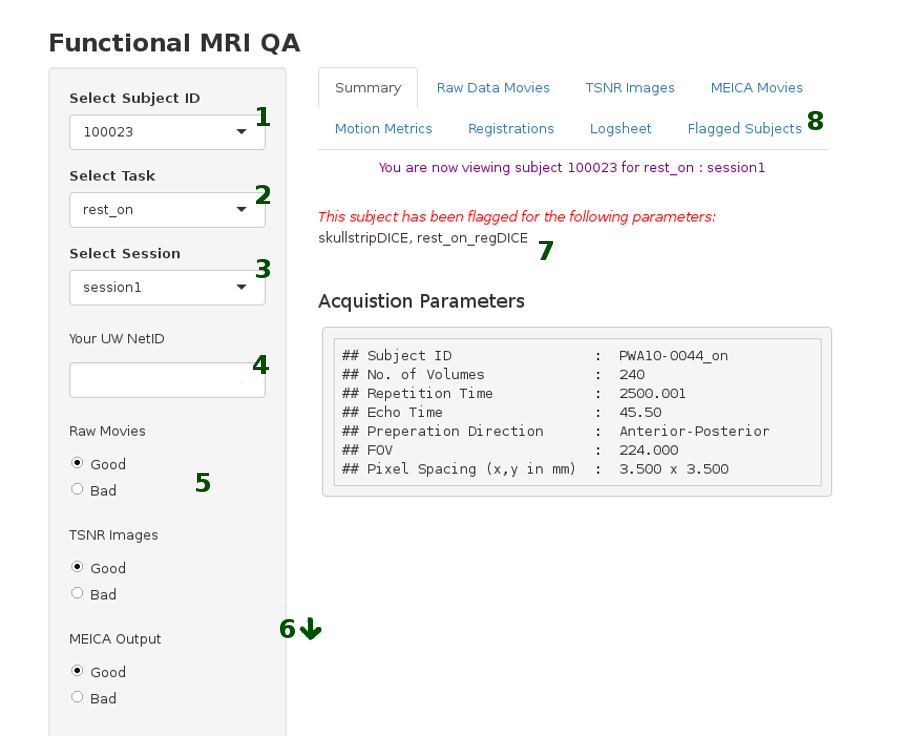
\includegraphics[scale=0.5]{shiny_summary_numbered.png}

\begin{enumerate}
	\item \textbf{Subject ID}: This is a drop-down menu that lists the subjects available for QA.
	\item \textbf{Tasks}: ``Tasks'' may include resting-state fMRI or breathhold fMRI, or some other task fMRI.
	\item \textbf{Session}: Currently, all subjects have only session1; if the study in longitudinal, more sessions will be added as the study progresses.
	\item \textbf{UW NetID}: Input your NetID here. This is necessary so we can keep track of the individuals who are looking at the QA reports. This will be submitted along with your comments to the QA logsheet.
	\item \textbf{Good/Fair/Bad}: For each measure, find the corresponding tab and select ``good'', ``bad'', or ``fair'' based on quality of the data. 
	\item \textbf{Submit a log}: Scroll down to the bottom of the sidebar, and click SUBMIT. If you accidentally submit an incorrect log, go to ShinyQA/output/ and remove your most recent entry. 
	\item \textbf{Warnings}: If warnings show up, pay especially close attention to the parameters or data that are flagged. These images are more likely to be problematic.
	\item \textbf{Flagged Subjects}: This tab lists all subjects that have data that has been flagged. 
\end{enumerate}

Next, we will take a look at how to distinguish between ``good'' and ``bad'' images. 

\section{Checking the Quality of Data}

In the section, we show some examples of bad and good images. The bad images may need to be re-preprocessed. 
\\
\\
\large{\textbf{Raw Data Movies:}}
\\\\
\noindent\begin{minipage}{0.45\textwidth}
	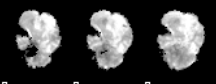
\includegraphics[scale=0.85]{bad_image2.png}
\end{minipage}%
\hfill%
\begin{minipage}{0.45\textwidth}
	\underline{\textbf{NOT an issue:}} Significant chunks of the brain are omitted in some of the movies. This is because of the way the brain is sliced, and does not need to be fixed.
	\\
\end{minipage}\newline\newline

\noindent\begin{minipage}{0.45\textwidth}
	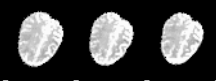
\includegraphics[scale=0.9]{bad_image3.png}
\end{minipage}%
\hfill%
\begin{minipage}{0.45\textwidth}
	\underline{\textbf{Issue:}} The brain is significantly tilted. \\
	\underline{\textbf{Fix:}} Make sure that the brain has been reoriented to standard space. 
\end{minipage}\newline\newline

\noindent\begin{minipage}{0.45\textwidth}
	
\includegraphics[scale=1.3]{bad_image5.png}
\end{minipage}%
\hfill%
\begin{minipage}{0.45\textwidth}
	\underline{\textbf{Issue:}} A movie show wrap-around effects as it runs. \\
	\underline{\textbf{Fix:}} See documentation on how to fix multiecho reconstruction failure erros on UDALL dropbox.
\end{minipage}\\\\\\
\noindent\begin{minipage}{0.45\textwidth}
	This is a usable image. No artifacts are present, and the whole brain is represented.
\end{minipage}%
\hfill%
\begin{minipage}{0.45\textwidth}
	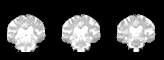
\includegraphics[scale=1.2]{meica_good2.png}
\end{minipage}
\\\\\\
\large{\textbf{TSNR:}}
\\\\
Bad TSNR images may appear blurred. Contrast may be incorrectly adjusted so that distinct brain structures are indistinguishable. \\\\
\noindent\begin{minipage}{0.45\textwidth}
	Brain structures are clear, and there is no obvious blurring. This is a good image.
\end{minipage}%
\hfill%
\begin{minipage}{0.45\textwidth}
	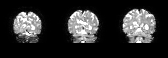
\includegraphics[scale=1.25]{tsnr_good2.png}
\end{minipage}\\\\
\noindent\begin{minipage}{0.45\textwidth}
	This is a good image. Contrast here is good, with clarity in regards to brain structures. 
\end{minipage}%
\hfill%
\begin{minipage}{0.45\textwidth}
	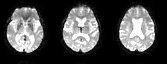
\includegraphics[scale=1.25]{tsnr_good1.png}
\end{minipage}
\\\\\\\\
\large{\textbf{Registration:}}
\\\\
\noindent\begin{minipage}{0.45\textwidth}
	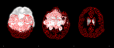
\includegraphics[scale=1.75]{badreg3.png}
\end{minipage}%
\hfill%
\begin{minipage}{0.45\textwidth}
	\underline{\textbf{Issue:}} Registration appears to barely try matching the actual brain. \\
	\underline{\textbf{Fix:}} Re-run the registration processing. If the tracing is still terribly off, PROC
\end{minipage}\newline\newline

\noindent\begin{minipage}{0.45\textwidth}
	Registration looks \emph{about} right. This image is acceptable. 
\end{minipage}%
\hfill%
\begin{minipage}{0.45\textwidth}
	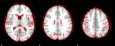
\includegraphics[scale=1.7]{reg_good1.png}
\end{minipage}\newline\newline
\noindent\begin{minipage}{0.45\textwidth}
	Registration follows the brain's contours fairly accurately. This image is good. 
\end{minipage}%
\hfill%
\begin{minipage}{0.45\textwidth}
	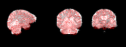
\includegraphics[scale=1.55]{reg_good2.png}
\end{minipage}
\newpage
\noindent\textbf{Other issues to look out for:}\\\\
\noindent\begin{minipage}{0.3\textwidth}
	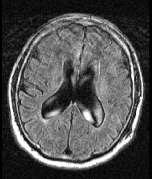
\includegraphics[scale=0.75]{T1_bad1.png}
\end{minipage}%
\hfill%
\begin{minipage}{0.6\textwidth}
	T1 images: Some ringing and blurriness can be perceived in the brain. This is due to motion during the T1 scan. No fix is currently available. 
\end{minipage}\\\\
\noindent\begin{minipage}{0.3\textwidth}
	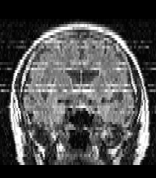
\includegraphics[scale=0.735]{T1_bad2.png}
\end{minipage}%
\hfill%
\begin{minipage}{0.6\textwidth}
	T1 images: Noise from the scanner itself appear on the image. Nothing can be done about these static-y artifacts, so this image is unusable. 
\end{minipage}
\\\\
\newline
For even more examples of what can go wrong with brain images, see \href{http://cbs.fas.harvard.edu/usr/mcmains/CBS_MRI_Quality_Control_Workshop.pdf}{\color{cyan}{this}}.

\section{Warnings}
\noindent\textbf{Skullstrip \& Registration DICE:} \\
e.g. skullstripDICE, rest\_on\_regDICE\\
For Skullstrip DICE, the warning indicates that the process of separating skull from brain in T1 images might not have been entirely successful. For registration DICEs, the warning indicates that the registration of the fMRI images to MNI space or study-specific template spaces are not very good and may need to be redone via some other method.\\\\

\textbf{Motion Metrics:} \\
e.g. axcpt\_on\_dvarsvals\_e002\_mean, abs\_mean\_displacement, percent\_outliers\\
 Warnings generated for motion metrics are primarily an indication that something may be wrong with task-relevant brain images due to too much motion; in movies, look for excessive motion. In still images, look for blurriness. 
 
\textbf{Scan Parameters:} \\
e.g. ME\_RS\_off\_slices, ME\_Task\_on\_echoes\\
These warnings indicate that the scan acquisition parameters for this subject's scan were incorrectly set or different from what they should be.\\\\

\section{Updating/Adding Warnings to the App}

Each subject's warnings appear near the top of their summary page. Additionally, warnings for all subjects can be observed in the flagged subjects tab. These warnings are read from the file \texttt{QA/\textbf{SUBJECTID}\_QA\_stats.csv} from each subject's directory. The file is structured as follows:
\begin{align*}
	& \texttt{measure,data,flag}\\
	& \texttt{RS\_off\_slices,37,0}\\
	& \texttt{RS\_off\_echoes,3,0}\\
	& \texttt{RS\_off\_dyn\_scans,240,0}\\
	& \texttt{RS\_off\_FOV\_RL,224.000,0}\\
	& ...
\end{align*}
and so on. When a flag = 1 (see third column), the corresponding measure's name is displayed in the app as a warning. The data column contains the measure's quantitative value.

To generate these .csv files, run \texttt{make QA/\textbf{SUBJECTID}\_QA\_stats.csv} from the terminal from each subject's directory. Alternatively, one can also call the \texttt{generate\_QA\_stats} script directly with two arguments \texttt{SUBJECTID} and \texttt{SESSIONNO} where the latter is the desired session number. Here is the default location of the QA csv-generating script:
\begin{center}
	\texttt{/mnt/panuc/IBIC\_Pipelines/ShinyQA/generate\_QA\_stats}
\end{center}

\textbf{Altering flag thresholds:} All thresholds are defined at the beginning of the script. To change the thresholds, simply edit these existing fields and regenerate all subjects' csv files after the update.

\textbf{Adding potential warnings:} Follow the output format (measure,data,flag) as shown above when adding to the script \texttt{generate\_QA\_stats}. This script generates flags in two stages, for task-independent and then task-dependent measures. Measures are task-dependent if they can be categorized as either \texttt{rest\_on}, \texttt{rest\_off}, \texttt{axcpt\_on}, or \texttt{axcpt\_off}. Add flag computations under the appropriate stage. Then re-generate the csvs for all subjects under the new script. 

\textbf{Future Improvements:} Whenever a QA stats csv file is updated, it is regenerated from scratch. As the flags being generated are currently inexpensive to compute, regeneration is quick. However, if more time-consuming flags are to be computed in the future, it would be a good idea to look into caching such flags in such a way that they need not be recomputed. 

\end{document}
